\section{Designs}
\subsection{System Design}
\subsubsection{Class diagrams and mind map}
The class structure design process started with a mind map to initially appraise the connection between each musical symbol. This helped break down a piece from a musician's view, and showed what information would be necessary between each symbol's class.

An initial class diagram was drawn from the mind map. This was modified during the course of development, testing and research of the initial model. In particular, other sources such as Music21 were looked at, a toolkit for computer-aided musicology \parencite{Music21}, which helped to examine whether the initial model was missing any classes or attributes. Furthermore, development showed that particular methods, such as the toString method and the Lilypond method could be improved by using inheritance from base classes in order to avoid unnecessary code duplication. The diagrams described are in the appendices. 
\subsection{UI Design}
The User interface for this project is designed after looking at the user interfaces used by other music applications. In particular, the developer was inspired by Spotify, shown in figure \ref{fig:spotify}.

\begin{figure}[h]
    \centering
    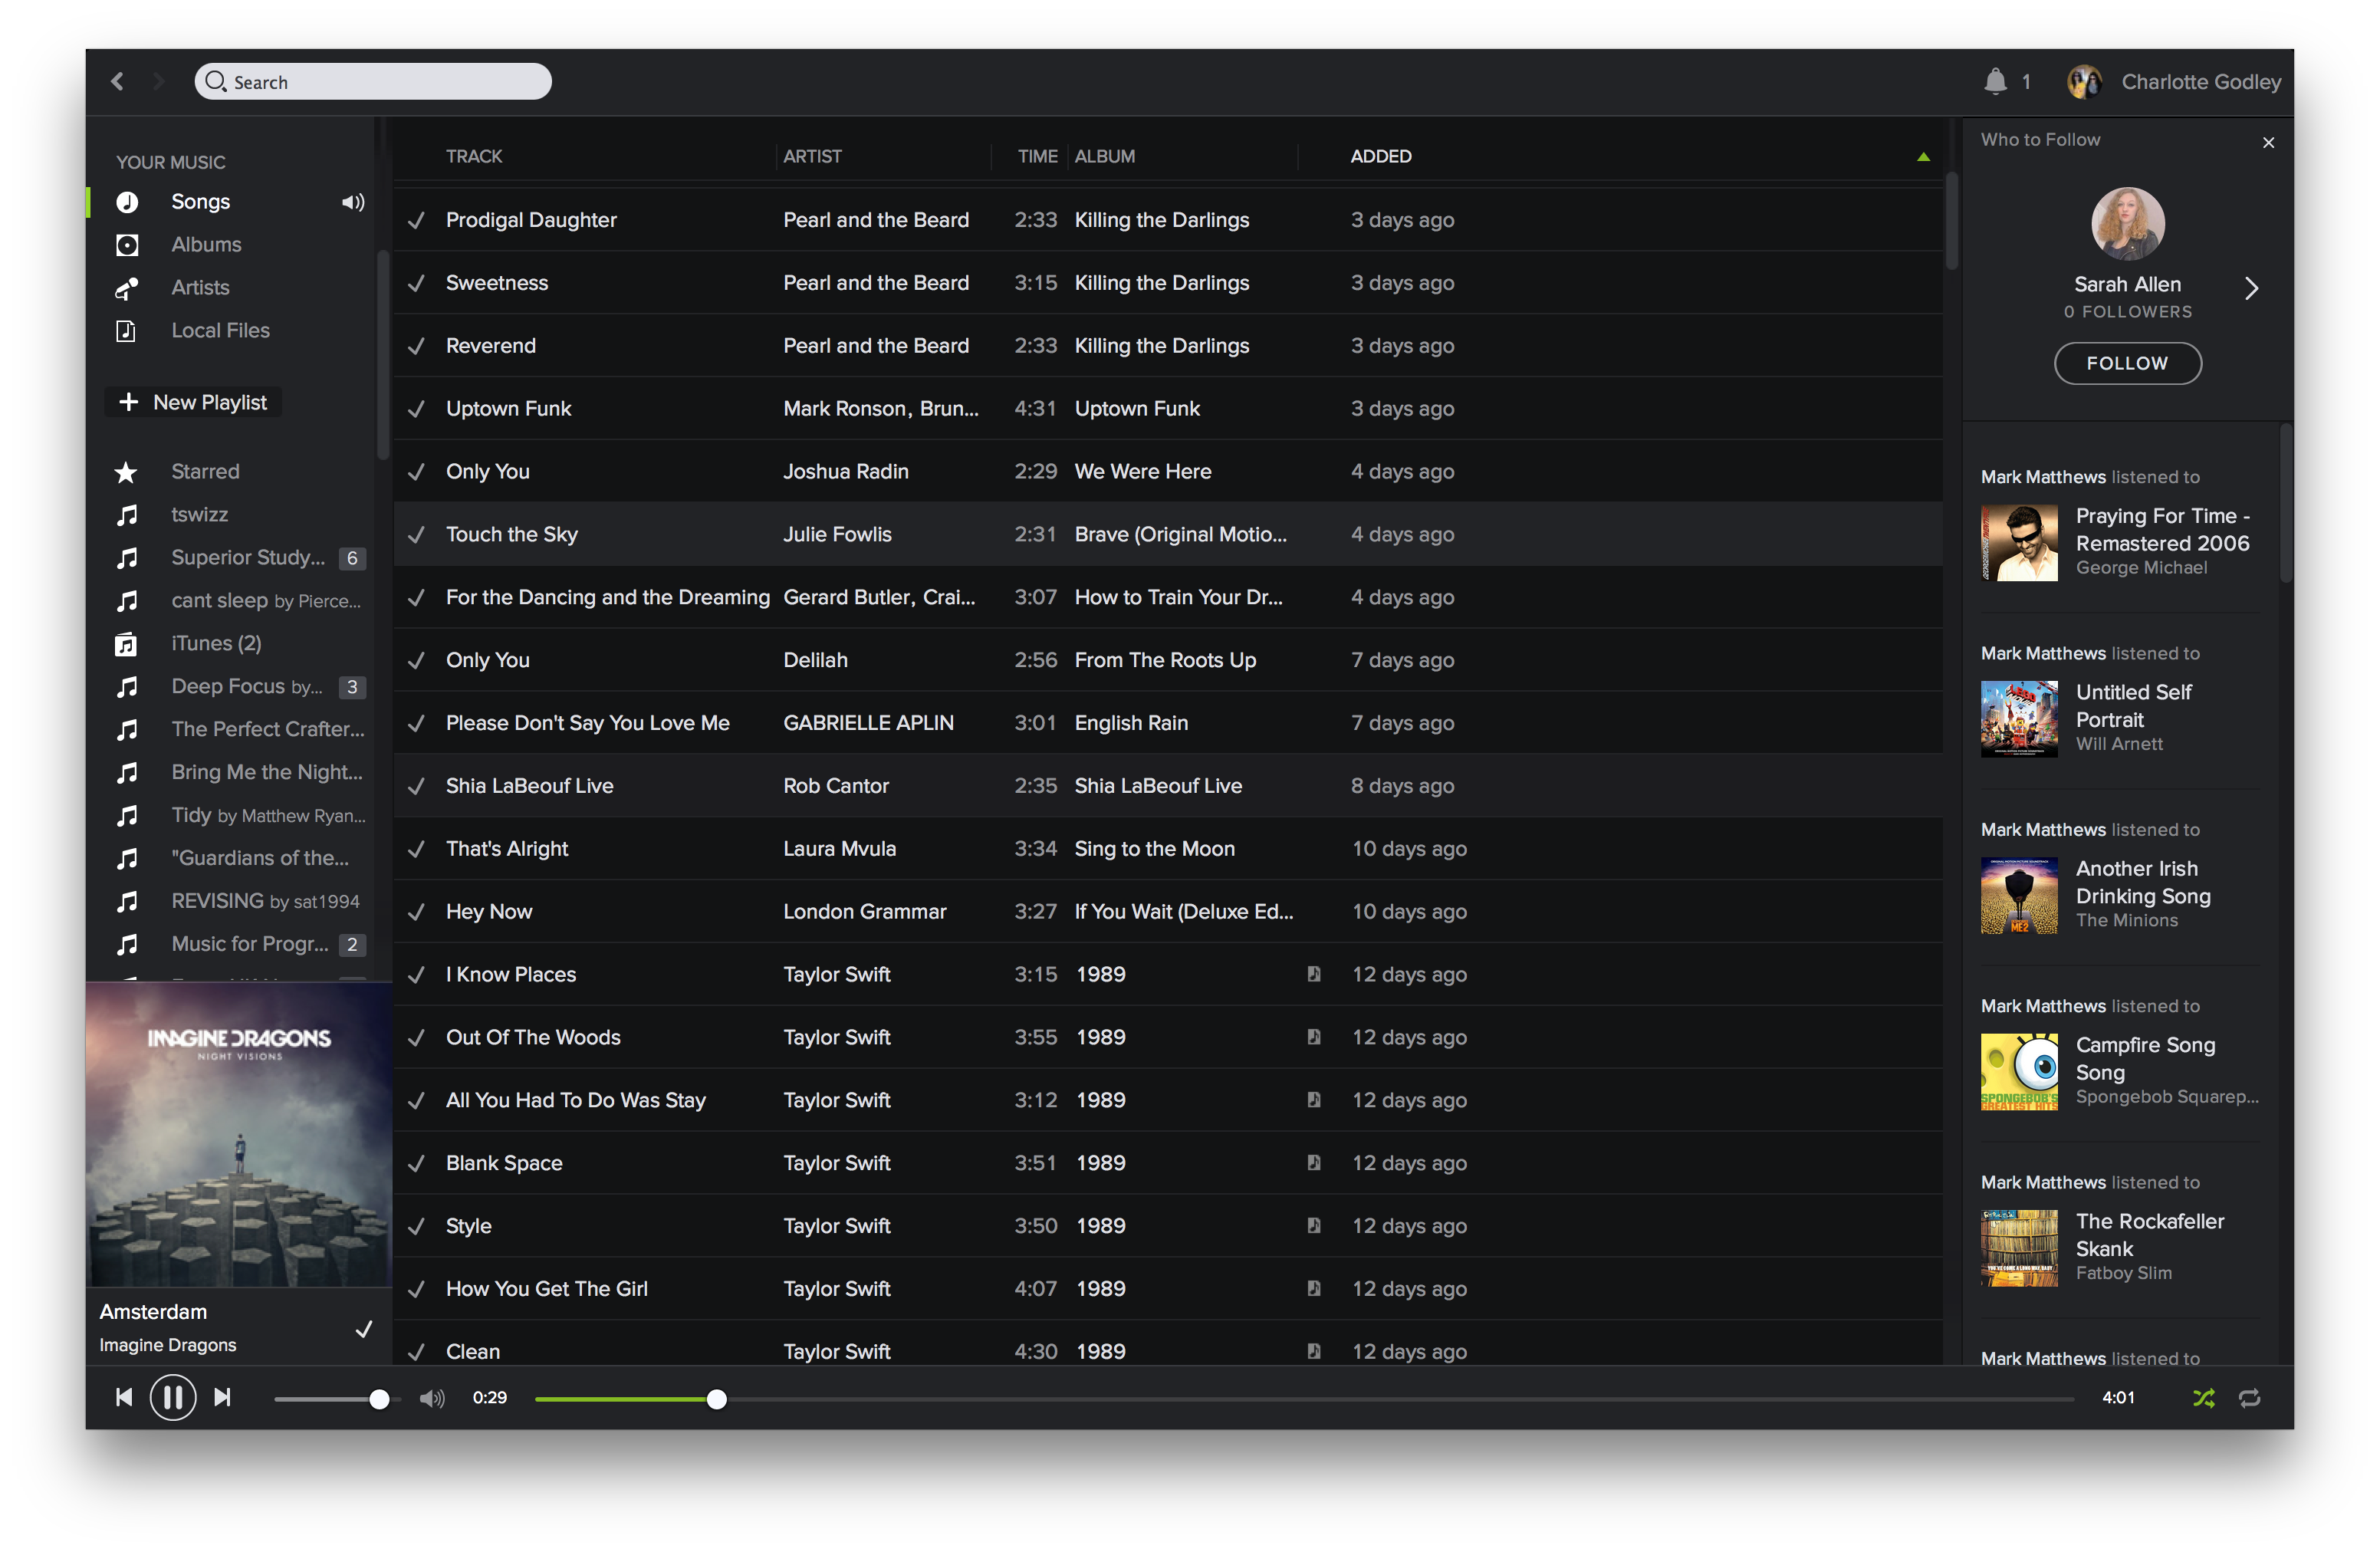
\includegraphics[width=\textwidth]{screen.png}
    \caption{Spotify user interface}
    \label{fig:spotify}
\end{figure}
\subsubsection{Main Display}
\begin{figure}[H]
    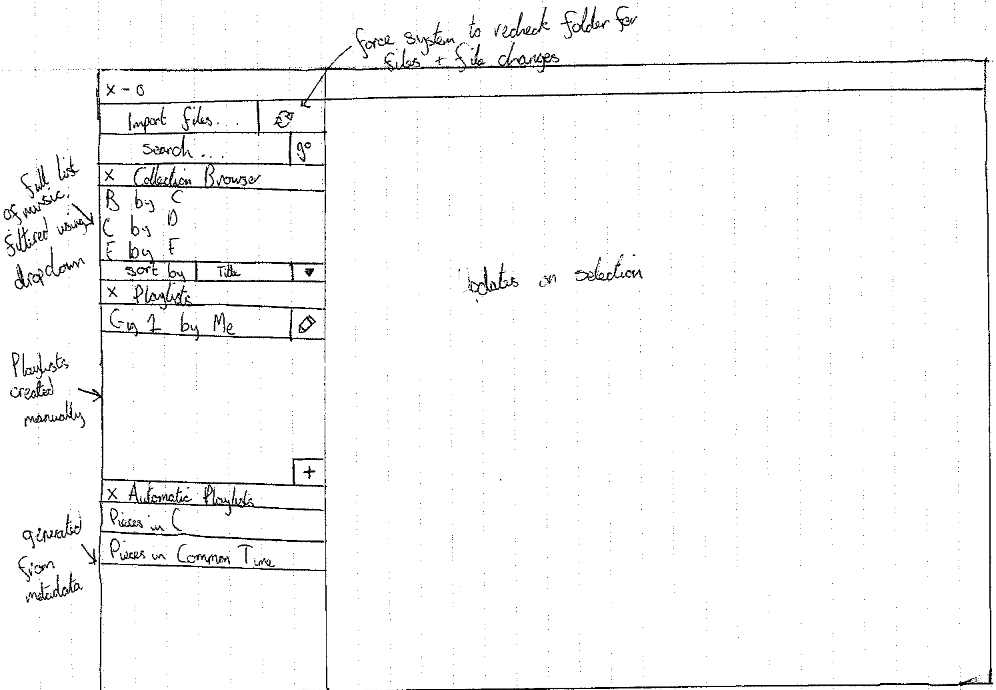
\includegraphics[width=400pt]{designs/main}
    \caption{Main User interface of the project}
    \label{fig:main}
\end{figure}
Figure \ref{fig:main} shows the main view of the application. Various panes to the left can be closed using the X button and show different ways the music can be displayed, either as individual units or as playlists. The larger pane next to it shows the area in which sheet music or a list of pieces in a playlist will be displayed, depending on the selection from the left pane. Updates to this and pop up boxes displaying dependent on buttons in the window are displayed and explained in the appendices.
\subsubsection{Musician feedback survey}
In order to understand how well this user interface works with a variety of users, a survey was designed which will be given to a selection of musicians, who will feedback on how easy the UI is to use and any updates which should be made to improve it. This feedback session will be performed after the initial sketches are made into a virtual user interface with no back end connected to the buttons. An example survey is provided in the appendices.
\subsection{Test Design}
This project will be developed using Test Driven Development. This is an Agile software development methodology which utilises the rules that a line of code should not be written unless there is a failing automated test \parencite{TDD}. This methodology has been chosen as the nature of the notation of music means that meticulous detail must be payed to how and with what symbol every element is notated, and Test Driven Development will significantly improve the quality of the software by closely integrating testing with the development process.

Development of tests and production code are ongoing, and as such the tests confirm critical, but self-contained units are correct, such as an accent being added to a measure correctly, or a note's pitch being created with a particular note name or octave number.

Test cases were created using the aforementioned software MuseScore. These were produced by creating a file for every area of notation (e.g. clefs, time signatures, note durations, pitch) and applying each and every symbol possible within that area to the music. It was decided to create test cases in this way to thoroughly ensure that no piece of notation was missed. An example testcase, and a list of all testcases in use and their value in real world testing, are included in the appendices.